
% This LaTeX was auto-generated from an M-file by MATLAB.
% To make changes, update the M-file and republish this document.

%%% \documentclass{article}
%%% \usepackage{graphicx}
%%% \usepackage{color}

%%% \sloppy
%%% \definecolor{lightgray}{gray}{0.5}
\setlength{\parindent}{0pt}

%%% \begin{document}

    
    
\subsection*{Integral Non Linearity of ADC}

\begin{par}
Example for algorithm INL
\end{par} \vspace{1em}
\begin{par}
INL is an algorithm for estimating Integral Non-Linearity of an ADC. ADC has to sample sinewave, ADC codes are required.
\end{par} \vspace{1em}
\begin{par}
See also 'Virosztek, T., Pálfi V., Renczes B., Kollár I., Balogh L., Sárhegyi A., Márkus J., Bilau Z. T., ADCTest project site: \url{http://www.mit.bme.hu/projects/adctest} 2000-2014';
\end{par} \vspace{1em}

\subsubsection*{Contents}

\begin{itemize}
\setlength{\itemsep}{-1ex}
   \item Generate sample data
   \item Call algorithm
\end{itemize}


\subsubsection*{Generate sample data}

\begin{par}
Suppose a sine wave of nominal frequency 10 Hz and nominal amplitude 1 V is sampled by ADC with bit resolution of 4. First quantities \lstinline{t} with time of samples and quantity \lstinline{bits} with number of bits are prepared and put into input data structure \lstinline{DI}.
\end{par} \vspace{1em}
\begin{lstlisting}[style=mcode]
DI = [];
DI.t.v=[0:1/1e4:1-1/1e4];
DI.bits.v = 4;
\end{lstlisting}
\begin{par}
Waveform is constructed.
\end{par} \vspace{1em}
\begin{lstlisting}[style=mcode]
Anom = 1; fnom = 2; phnom = 0;
wvfrm = Anom*sin(2*pi*fnom*DI.t.v + phnom);
\end{lstlisting}
\begin{par}
Next code values are calculated. It is simulated by quantization and scaling of the sampled waveform. In real measurement code values can be obtained directly from the ADC. Suppose ADC range is -1..1.
\end{par} \vspace{1em}
\begin{lstlisting}[style=mcode]
codes = wvfrm;
rmin = -1; rmax = 1;
levels = 2.^DI.bits.v - 1;
codes(codes<rmin) = rmin;
codes(codes>rmax) = rmax;
codes = round((codes-rmin)./2.*levels);
\end{lstlisting}
\begin{par}
Now lets introduce ADC error. Instead of generating code 2 ADC erroneously generates code 3 and instead of 10 it generates 11.
\end{par} \vspace{1em}
\begin{lstlisting}[style=mcode]
codes(codes==2) = 3;
codes(codes==10) = 11;
codes = codes + min(codes);
\end{lstlisting}
\begin{par}
Create quantity \lstinline{codes} and plot a figure with sampled sine wave and codes.
\end{par} \vspace{1em}
\begin{lstlisting}[style=mcode]
DI.codes.v = codes;
figure
%plot(t, (y+1).*1/2.*levels, t, codes);
hold on
stairs(DI.t.v, codes);
wvfrm = (wvfrm + Anom).*levels./2;
plot(DI.t.v, wvfrm, '-r');
xlabel('t (s)')
ylabel('Codes / Voltage (scaled)');
legend('Codes generated by ADC','Original waveform scaled to match codes');
hold off
\end{lstlisting}

\begin{center}
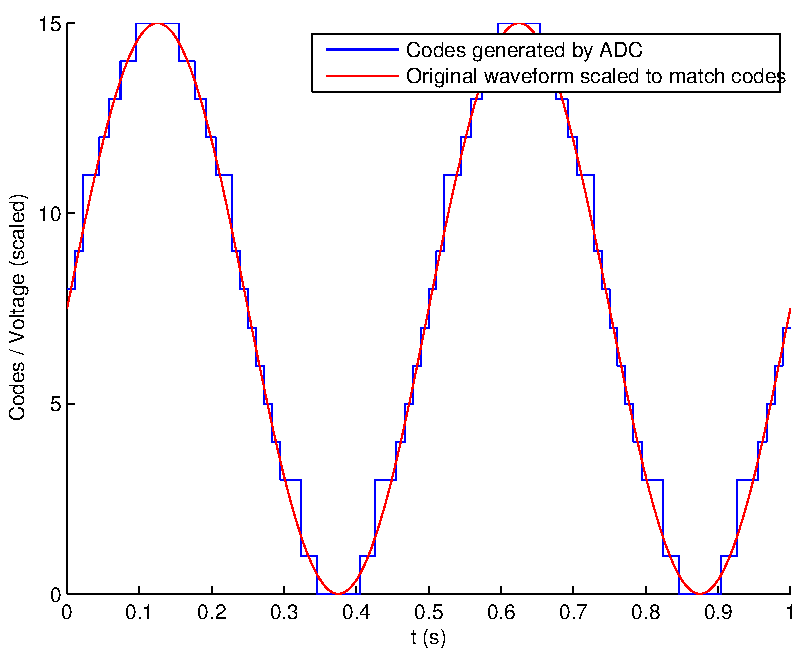
\includegraphics[width=0.7\textwidth]{alg_examples_published/INL_alg_example_01.pdf}
\end{center}


\subsubsection*{Call algorithm}

\begin{par}
Apply INL algorithm to the input data \lstinline{DI}.
\end{par} \vspace{1em}
\begin{lstlisting}[style=mcode]
DO = qwtb('INL', DI);
\end{lstlisting}

        \begin{lstlisting}[style=output]
QWTB: no uncertainty calculation
\end{lstlisting} \color{black}
    \begin{par}
Plot results of integral non-linearity. One can clearly observe defects on codes 3 and 11.
\end{par} \vspace{1em}
\begin{lstlisting}[style=mcode]
figure
plot(DO.INL.v, '-x');
xlabel('Code value')
ylabel('INL')
\end{lstlisting}

\begin{center}
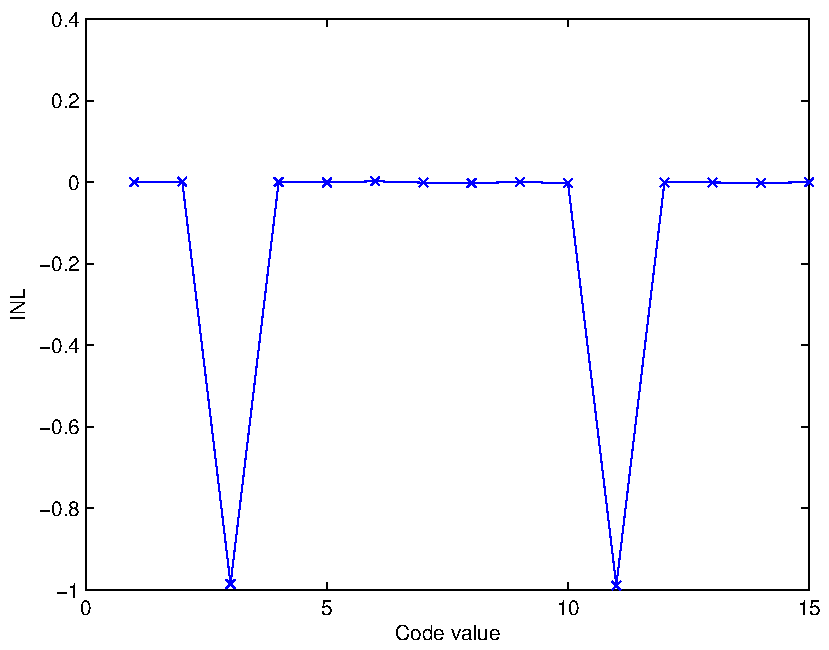
\includegraphics[width=0.7\textwidth]{alg_examples_published/INL_alg_example_02.pdf}
\end{center}



%%% \end{document}
    
